% !TEX root = template.tex

\section{Results}
\label{sec:results}

The \gls{ars} previously described has been tried on a PC with an Intel Core i7-7700HQ microprocessor at 3.8 GHz, 8 GB of RAM, and an NVIDIA Ge-Force GTX 1050 as Graphic Card. The programming language used was Python with Keras and TensorFlow as learning framework. The most computational demanding operations was performed on the GPU using CUDA drivers.
The learning part has been tried also performing all the computations on the CPU, the difference in time is dramatically: using the GPU each epoch takes about 26 seconds while using only CPU takes more than 2 minutes.

In the learning phase, the training accuracy reaches $93.75\%$ while in the test dataset, activities are recognized the $94.6\%$ of the time.

Once the model has been learned, the \gls{cnn} is used to predict activities in real time. To assess the performance of this task, a set of predictions has been made on a raw signal recorded by the same sensor. The overall recognition rate of the real time prediction is $75.88\%$, precision and recall are showed in \fig{fig:precision} and \fig{fig:recall}.

The accuracy in the prediction phase is quite low, since the dataset used is too small and has a great variance within the data. Moreover in that dataset some labels are missing.

As can be seen the accuracy is very good for longer or easy-to-recognize activities like \textit{running}, \textit{walking}, \textit{standing} and \textit{lying}, while is lower for shorter activities or activities that suffer of a big variance such as \textit{falling} and \textit{sitting}.

In \cite{Korbinian} precision and recall are plotted only for the main activities, they don't take into account the transition activities (\textit{up}, \textit{down}, \textit{ascending}, \textit{descending}). These activities give a low accuracy since they have less samples in the dataset and since they can have an high variance.

\begin{figure}
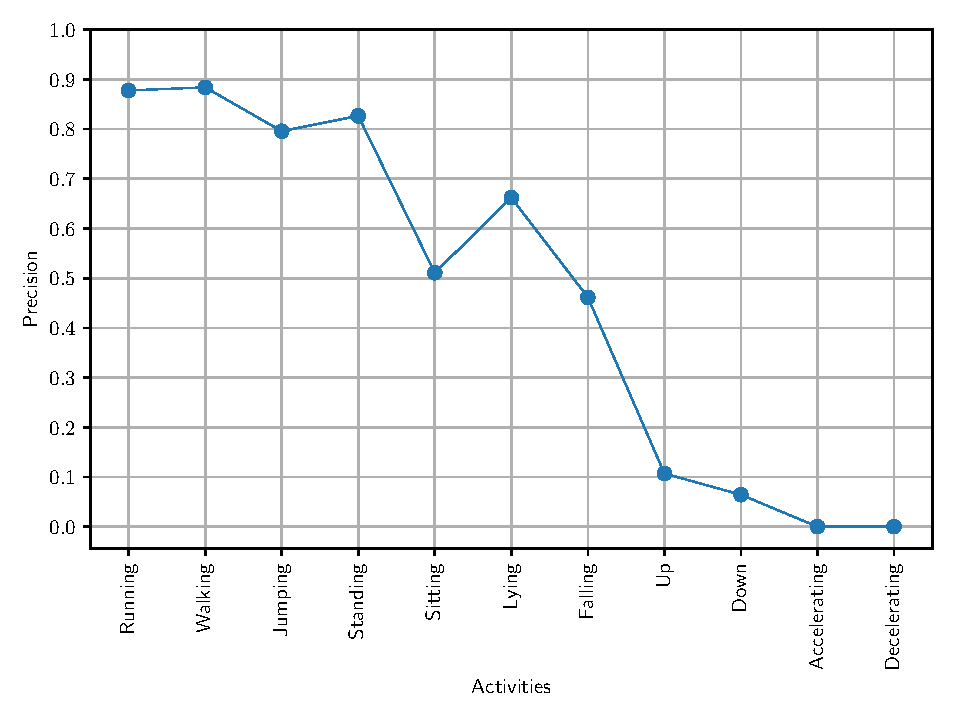
\includegraphics[scale=0.55]{precision.pdf}
\caption{Precision calculated for each activity to recognize}
\label{fig:precision}
\end{figure}

\begin{figure}
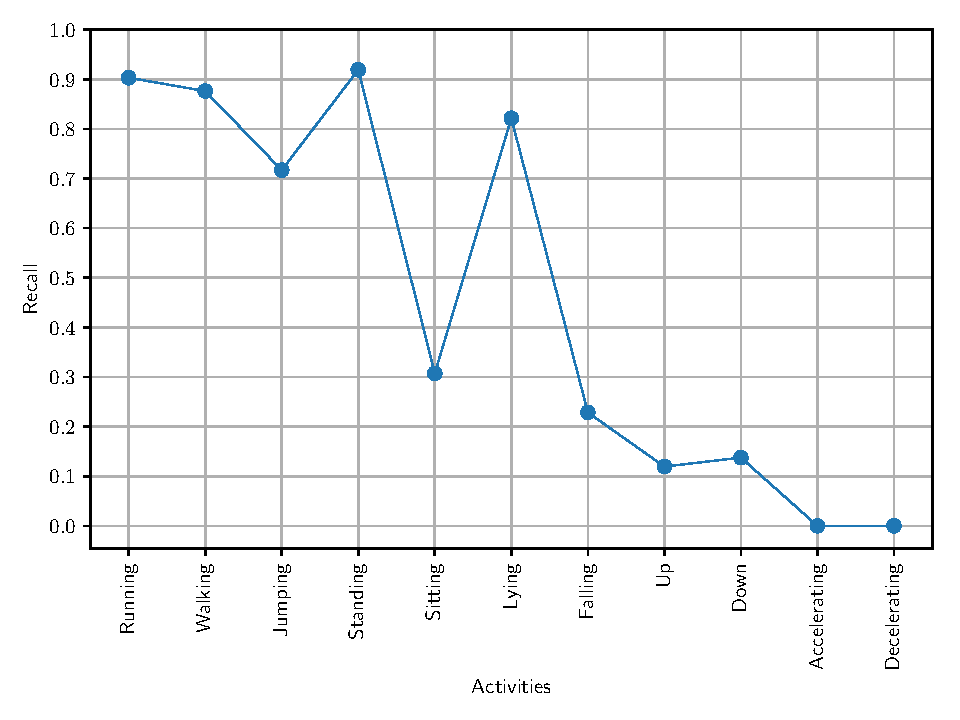
\includegraphics[scale=0.55]{recall.pdf}
\caption{Recall calculated for each activity to recognize}
\label{fig:recall}
\end{figure}